%%%%%%%%%%%%%%%%%%%%%%%%%%%%%%%%%%%%%%%%%
% The Legrand Orange Book
% LaTeX Template
% Version 1.2 (19/5/13)
%
% This template has been downloaded from:
% http://www.LaTeXTemplates.com
%
% Original author:
% Mathias Legrand (legrand.mathias@gmail.com)
%
% License:
% CC BY-NC-SA 3.0 (http://creativecommons.org/licenses/by-nc-sa/3.0/)
%
% Compiling this template:
% This template uses biber for its bibliography and makeindex for its index.
% This means that to update the bibliography and index in this template you
% will need to run the following sequence of commands in the template
% directory:
%
% 1) pdflatex main
% 2) makeindex main.idx -s StyleInd.ist
% 3) biber main
% 4) pdflatex main
%
% This template also uses a number of packages which may need to be
% updated to the newest versions for the template to compile. It is strongly
% recommended you update your LaTeX distribution if you have any
% compilation errors.
%
% Important note:
% Chapter heading images should have a 2:1 width:height ratio,
% e.g. 920px width and 460px height.
%
%%%%%%%%%%%%%%%%%%%%%%%%%%%%%%%%%%%%%%%%%

%----------------------------------------------------------------------------------------
%	PACKAGES AND OTHER DOCUMENT CONFIGURATIONS
%----------------------------------------------------------------------------------------

\documentclass[11pt,fleqn,openany]{book} % Default font size and left-justified equations

\usepackage[top=2cm,bottom=2cm,left=2.5cm,right=2.5cm,headsep=10pt,a4paper]{geometry} % Page margins

\usepackage{xcolor} % Required for specifying colors by name
\definecolor{red}{RGB}{173,26,31} % Define the blue color used for highlighting throughout the book
\definecolor{grey}{RGB}{47,49,51} % Define the blue color used for highlighting throughout the book

\usepackage{array}
\newcolumntype{C}[1]{>{\centering\arraybackslash}p{#1}}
\usepackage{multirow}

% Font Settings
\usepackage{avant} % Use the Avantgarde font for headings
%\usepackage{times} % Use the Times font for headings
\usepackage{mathptmx} % Use the Adobe Times Roman as the default text font together with math symbols from the Sym­bol, Chancery and Com­puter Modern fonts

\usepackage{microtype} % Slightly tweak font spacing for aesthetics
\usepackage[utf8]{inputenc} % Required for including letters with accents
\usepackage[T1]{fontenc} % Use 8-bit encoding that has 256 glyphs

% Index
\usepackage{calc} % For simpler calculation - used for spacing the index letter headings correctly
\usepackage{makeidx} % Required to make an index
\makeindex % Tells LaTeX to create the files required for indexing

\usepackage{listings}
\usepackage{textcomp}

% Taken from http://www.monperrus.net/martin/copy-pastable-listings-in-pdf-from-latex
\lstset{
upquote=true,
columns=fullflexible,
keepspaces=true,
basicstyle=\footnotesize\ttfamily,
literate={*}{{\char42}}1
         {-}{{\char45}}1
}

%----------------------------------------------------------------------------------------

\input{./structure.tex} % Insert the commands.tex file which contains the majority of the structure behind the template

% Define Cloud Gateway version
\newcommand{\cgversion}{1.1.2}
% Define Configuration references command
\newcommand{\cgconfigreference}[1]{See \textit{\nameref{config:#1}} on page~\pageref{config:#1}.}

\begin{document}

%----------------------------------------------------------------------------------------
%	TITLE PAGE
%----------------------------------------------------------------------------------------

\begingroup
\thispagestyle{empty}
\AddToShipoutPicture*{\put(0,0){\includegraphics[scale=1]{background_nuage2.png}}} % Image background
%\centering
\vspace*{22cm}
\par\normalfont\fontsize{30}{30}\sffamily\selectfont\color{white}
\begin{tabular}{C{10cm}C{2cm}}
Cloud Gateway \\
- & \\
 Reference Manual & \\
\end{tabular}
%\vspace*{1cm}
%{\Huge Nuage Labs SAS}\par % Author name
\endgroup

%----------------------------------------------------------------------------------------
%	TABLE OF CONTENTS
%----------------------------------------------------------------------------------------

\chapterimage{chapter_head_background.jpg}

\pagestyle{empty} % No headers

\cleardoublepage % Forces the chapter to start on an odd page so it's on the right

\tableofcontents % Print the table of contents itself

\cleardoublepage % Forces the chapter to start on an odd page so it's on the right

\pagestyle{fancy} % Print headers again

\chapter{Introduction}
\label{chap:introduction}

Cloud Gateway is a software gateway turning any Cloud storage service\footnote{Compatible with the Amazon S3 or Openstack API.} into a local volume.
No API integration is required, data are stored on the Cloud, encrypted during transfers and can be replicated between multiple Clouds.\\

Your Cloud storage area works as a local filesystem,
which can be exported to the network as a NAS\footnote{Network-Attached Storage} through standards protocols like NFS\footnote{Network File System.} or CIFS\footnote{Common Internet File System.},
enabling the transparent use of all the Cloud storage features without any modifications to exsiting applications or any vendor lockup.

\section{Features}
\label{sec:features}

\subsection{Flexible, on demand and cost-effective cloud storage}

A key advantage in using Cloud storage is the unlimited physical storage constraint. Your own local volume that could be mounted trough NFS thanks to Cloud Gateway can bear as much data as you would like to store. No saturation issue, no evolution issue, ttal flexibility, it's virtually infinite. And thanks to Cloud storage, you only pay for what you use. Your storage costs become fully flexible. You don’t need to invest in the acquisition of expensive storage solutions of several Tera-Bytes which will be under-used. No more storage limit and your storage costs is directly related to your need for expanded / reduced storage.

\subsection{No API, no development, no vendor lockup}

Using Cloud Gateway means there is no initial investment in API integration. Moving to Cloud storage is only a few clicks away without modifying the way your application is functioning in any way = Time \& Cost Efficiency.

\subsubsection*{The choice of Cloud storage providers is yours}

Once connected via Cloud Gateway, no source code modification of your software is required to integrate a proprietary API, therefore you keep your freedom. Switching Cloud storage provider is up to you and only one click away. You can also change back to a traditional local storage avoiding any technical issue. You are totally independent and are able to use competitive tension amongst providers to obtain best possible terms on your data storage.

\subsubsection*{No lock-up through a proprietary API}

Your own storage local volume is mounted through NFS (Network File System) or CIFS (Common Internet File System) on your own platform as though your storage is dealt with locally on your own network. Re-internalisation of your data is possible at any time without any technical or commercial difficulty.

\subsubsection*{Openness}

All data are retained in a fully transparent, accessible and documented format. You will choose our products because they are the best out there and not because you are stuck with them!

The Cloud Gateway concept is designed to release Cloud storage users from proprietary API and offer a standardised interface POSIX compatible which is accessible via standard and tested protocols such as FUSE, NFS or CIFS. Bearing this in mind, our products do not include a proprietary API and are fully based on standard protocols.

Our philosophy is to offer end users a maximum level of control on the product through a number of fully flexible and configurable parameters:
\begin{itemize}
\item Compression levels ;
\item Encryption algorithms ;
\item Optimal operation size (IO Block Size) ;
\item Timeouts duration at various levels (database access, HTTP(S) transfers etc.\\
\end{itemize}

All our configuration files are in XML format so as to be easily readable by a person as well as easily handled via scripts or external programs. These file formats are documented and are therefore unsurprisingly standard.

Because we are aware our products and services are to be used in complex environments, our products are designed to be able to interact with various classic monitoring tools such as Munin or Nagios.

\subsection{High availability}

The Nuage Labs team is composed of highly trained engineers with a long experience in complex architecture management with high availability constraints. This is why our products are designed with the dual objective of offering robustness, monitoring and fail-over systems in order to guarantee service continuity at all times.

\begin{figure}[H]
\centering
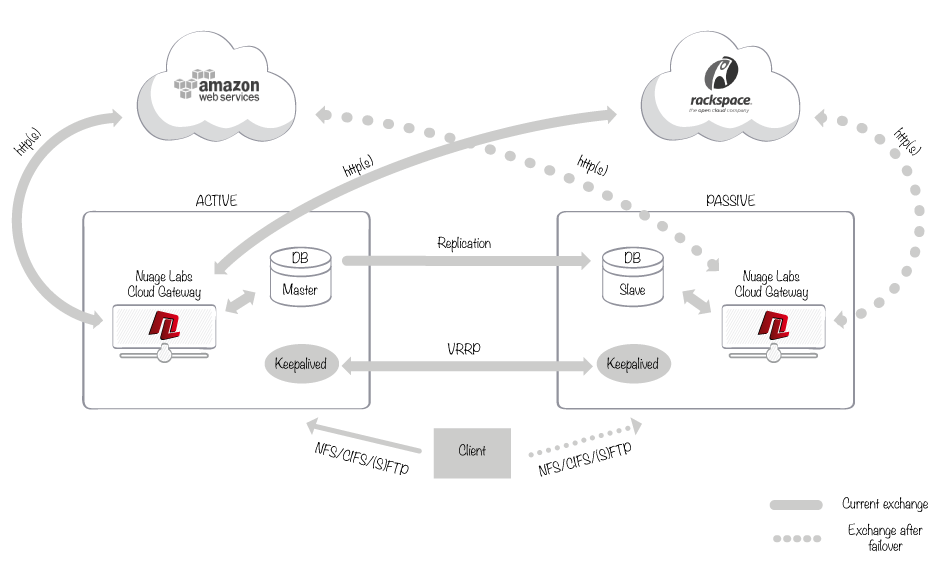
\includegraphics[width=1\textwidth]{cloud-gateway-redundancy.png}\\
High-Availability with Cloud Gateway
\end{figure}

The active / passive mode from Cloud Gateway, linked with a mirroring functionality from two separate Cloud storage providers offers an architecture without a point of failure\footnote{Single Point of Failure, or SPoF.}.

\subsection{Integrity}

Because we know your data are your most valuable asset, we have integrated various encryption mechanisms within our solutions in order to assess data integrity during data exchange with storage providers. When your provider’s technology allow it, we check data integrity by default as and when data are placed on the provider’s platform by comparing the imprint before data are sent to the Cloud, with the one recorded by the storage provider (usually MD5 format). We would also typically check data integrity when recovering the file from the storage provider.
The way your data are stored is simple, transparent and documented allowing you to repatriate them, should you choose to stop using our service.

\subsection{Confidentiality}

Cloud Gateway can ensure files confidentiality at all times during data transfers to the Cloud storage provider as well as during storage through a strong specific encryption based on tried and tested algorithms. Should you wish to, data transfers can be entirely performed via HTTPS and files can be encrypted at a level satisfying your own requirements:\\
\begin{itemize}
\item AES 128 bits ;
\item AES 192 bits ;
\item AES 256 bits ;
\item Blowfish 128 bits ;
\item Camellia 128 bits ;
\item Camellia 192 bits ;
\item Camellia 256 bits.\\
\end{itemize}

Cloud Gateway supports the most secure standards of SSL/TLS to secure your transfers, like TLS 1.0, 1.1 and 1.2, Perfect Forward Secrecy and Elliptic Curves.\\

File encryption is always done on the basis of block chains (Cipher Bloc Chaining or CTR Integer Counter Mode) with a salt and a unique and randomly generated initialization vector (IV) in order to guarantee a robust level of confidentiality. The encryption key is known only by you. Nuage Labs does not have access to your data and should you activate the data encryption, neither does the Cloud storage provider.

\subsection{Efficiency}

A question often raised on data accessibility through the Cloud is performance limitation while accessing files stored online. Cloud Gateway solves this key issue, integrating a cache mechanism to its solution. Although caches performance mostly depend on the equipment on which they are deployed as well as the allocated size, our team is proud to confirm that access performance are highly improved compared to a direct Cloud storage (access to files not being dependent upon DNS or HTTP(S) requests and not being constrained by bandwidth between your application and the Cloud storage provider.\\

According to data storage typology, our compression system as integrated to Cloud Gateway can reach factors close to 95\%.
The level of compression can easily be configured balancing out the quantity of space used at the storage provider level, data access time and CPU and memory charge available on your platform.\\

In order to avoid classic bottlenecks, Cloud Gateway uses an asynchronous event internal architecture with a low number of processes.
Each process is dedicated to its own task with a separate addressable memory and is monitored by a parent process whose sole role is to ensure other processes are correctly run.

The asynchronous architecture enables to avoid almost all drawbacks from a number of processes such as:
\begin{itemize}
\item thundering herd ;
\item lock contention ;
\item c10k problem.
\end{itemize}

The strict task slicing enables to limit modules and locks dependency allowing to fully benefit from modern multi-cores architectures.\\

\cleardoublepage % Forces the chapter to start on an odd page so it's on the right

\chapter{Installation}
\label{chap:installation}

%% There are currently two ways to install Cloud Gateway on a server:\\
There is currently only one way to install Cloud Gateway on a server:\\
\begin{itemize}
%% \item using a .deb package ;
\item compiling it from source.\\
\end{itemize}

%%While the first way is clearly the easiest one for users of a Debian-based Linux distribution (Debian, Ubuntu,~...)
%% with administrator privileges, the second one allows more flexibility in the way Cloud Gateway is deployed and supports virtually all Linux flavors.\\

\section{Technical requirements}
\label{sec:technical-requirements}

For the machine (either virtual or bare-metal) on which Cloud Gateway is to be deployed, the following requirements shall be met:\\
\begin{itemize}
\item a Linux 64 bits kernel >= 2.6.32 ;
\item a Bash shell >= 3.0 ;
\item a PostgreSQL server >= 9.1 \footnote{the PostgreSQL server can be installed on an other host, or even on a cluster of hosts for maximum performance.} ;
\item a FUSE module\footnote{File System In Userspace, a kernel component available in all modern distributions.}.\\
\end{itemize}

At this time, Cloud Gateway has been successfully tested on the following Linux versions:\\
\begin{itemize}
\item Debian 7.0 (x86\_64) (Wheezy) ;
\item Debian 8.0 (x86\_64) (Jessie) ;
\item Ubuntu Server 12.04 (x86\_64) (LTS) ;
\item Ubuntu Server 13.04 (x86\_64) ;
\item Ubuntu Server 13.10 (x86\_64) ;
\item Ubuntu Server 14.04 (x86\_64) (TLS) ;
\item openSUSE 12.3 (x86\_64) (Dartmouth) ;
\item openSUSE 13.1 (x86\_64) (Bottle) ;
\item SUSE Linux Enterprise Server 11.2 (x86\_64) ;
\item CentOS 6.4 (x86\_64).\\
\end{itemize}

%% The installation via .deb package is only available on Debian or Ubuntu, and the exact name of the .deb package differs from version to version.\\

%% \section{Using the Debian / Ubuntu package}
%% \label{sec:debian-package}

%% The first step is to install the required dependencies of the Cloud Gateway package:

%% \begin{lstlisting}[language=bash]
%% $ sudo aptitude install fuse postgresql postgresql-client ca-certificates
%% \end{lstlisting}

%% then, simply installing the package itself:

%% \begin{lstlisting}[language=bash]
%% $ sudo dpkg -i CloudGateway-1.1.2-x86_64.deb
%% Selecting previously unselected package cloudgateway.
%% (Reading database ... 38931 files and directories currently installed.)
%% Unpacking cloudgateway (from .../CloudGateway-1.1.2-x86_64.deb) ...
%% Setting up cloudgateway (1.1.2-1) ...
%% Database user successfully created.
%% Tables successfully created.
%% Configuration successfully updated.
%% Database successfully created.
%% $
%% \end{lstlisting}

\section{Compilation}
\label{sec:compilation}

You can find the source on github : https://github.com/nuagelabsfr/cloud-gateway. Please follow the REAMDE instructions you will find in the repository.

\section{Cloud Gateway User}
\label{sec:cloud-gateway-user}

Because Cloud Gateway does not need any security privileges to run, Nuage Labs strongly advises to use a dedicated
system user instead of running Cloud Gateway as \textit{root}.\\

For that reason, the Debian package creates a new user named \textit{cloudgw} if it does not exist yet.
This user owns the Cloud Gateway files, and it is under its identity that Cloud Gateway should be run.

\cleardoublepage % Forces the chapter to start on an odd page so it's on the right
\chapter{Configuration}
\label{chap:configuration}

\section{Components overview}
\label{sec:components-overview}

\begin{figure}[H]
\centering
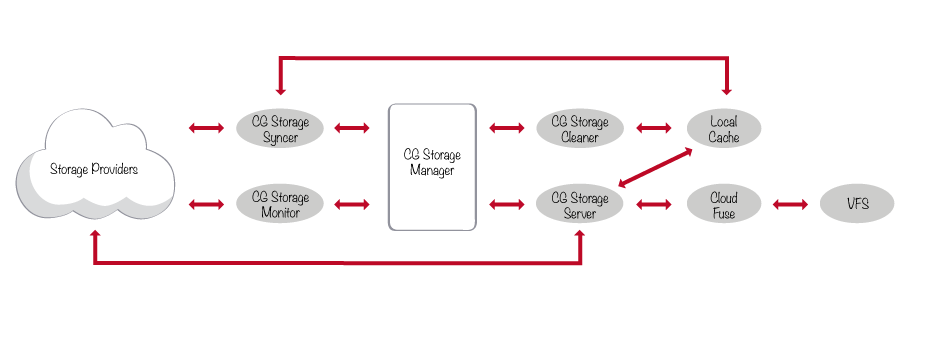
\includegraphics[width=1.1\textwidth]{schema-internal-01-01.png}\\
Cloud Gateway components overview
\end{figure}

Cloud Gateway's main component is the Storage Manager, a daemon handling accesses to the filesystem
and efficiently managing the communications with the cloud storage providers. The Storage Manager itself is composed
of 4 different processes:\\
\begin{itemize}
\item the Storage Server, handling filesystem's accesses ;
\item the Storage Cleaner, expunging unused files from the cache ;
\item the Storage Monitor, monitoring every storage provider in order to provides the best performances ;
\item and the Storage Syncer, syncing the files with the different storage providers.\\
\end{itemize}

\section{Configuring the Storage Manager}
\label{sec:configuring-the-storage-manager}

The Storage Manager associates one or many\footnote{More than one space are used in case of Striping or Mirroring.} storage spaces\footnote{Bucket in Amazon S3 terminology, container in Openstack.} to
a virtual filesystem. First the storage spaces, named {\color{red}Instances}, are defined, then {\color{red}filesystems}. At last, the mapping between filesystems and instances has to be configured.\\

{\color{red}Caution: A given instance should not be associated with more than one filesystem, otherwise collisions and data loss will occur.}

\subsection*{Adding a Cloud Storage provider instance}

Adding an {\color{red}Instance} is easy:\\

{\color{red}Caution: Note that the container / bucket should exist before the Storage Manager is started.}

\begin{itemize}

\item Openstack Swift Identity v1 (Rackspace,~...):
\begin{lstlisting}[language=bash]
$ /usr/local/bin/CloudGatewayAddInstance -n <Instance Name> \
  -P Openstack \
  -f /usr/local/etc/CloudGatewayConfiguration.xml \
  -i 1 -A <Authentication Endpoint> -c <Container Name> \
  -u <Username> -I <API Key>
\end{lstlisting}

\item Openstack Swift Identity v2 with a TenantName (CloudWatt, OVH,~...):
\begin{lstlisting}[language=bash]
$ /usr/local/bin/CloudGatewayAddInstance -n <Instance Name> \
  -P Openstack \
  -f /usr/local/etc/CloudGatewayConfiguration.xml \
  -i 2 -A <Authentication Endpoint> -c <Container Name> \
  -u <Username> -p <Password> -T <Tenant Name>
\end{lstlisting}

\item Openstack Swift Identity v2 with a TenantId (HP,~...):
\begin{lstlisting}[language=bash]
$ /usr/local/bin/CloudGatewayAddInstance -n <Instance Name> \
  -P Openstack \
  -f /usr/local/etc/CloudGatewayConfiguration.xml \
  -i 2 -A <Authentication Endpoint> -c <Container Name> \
  -u <Username> -p <Password> -t <Tenant Id>
\end{lstlisting}

\item S3 (Amazon, Scality, SFR, YaCloud,~...):
\begin{lstlisting}[language=bash]
$ /usr/local/bin/CloudGatewayAddInstance -n <Instance Name> \
  -P Amazon \
  -f /usr/local/etc/CloudGatewayConfiguration.xml \
  -e <Endpoint> -g <Endpoint Port> -S <false for HTTP, true for HTTPS> \
  -b <Bucket Name> -a <Key> -s <Secret>
\end{lstlisting}
\end{itemize}

Please take care of the fact that the Openstack \textbf{Authentication Endpoint} URL does not contain the final \textbf{/v1.0/}, \textbf{/v1.1/} or \textbf{/v2.0/} part that some providers
mention in their documentation, as it is automatically appended by Cloud Gateway.\\

Sample values for some common providers are available below, please
note that they may not be valid for your account:\\

\begin{tabular}{|l|l|}
\hline
\textbf{Provider} & \textbf{Endpoint}  \\
\hline
Amazon S3 (US Standard) & s3.amazonaws.com \\
Amazon S3 (US West Oregon) & s3-us-west-2.amazonaws.com \\
Amazon S3 (US West Northern California) & s3-us-west-1.amazonaws.com \\
Amazon S3 (EU Ireland) & s3-eu-west-1.amazonaws.com \\
Amazon S3 (Pacific Singapore) & s3-ap-southeast-1.amazonaws.com \\
Amazon S3 (Pacific Sydney) & s3-ap-southeast-2.amazonaws.com \\
Amazon S3 (Pacific Tokyo) & s3-ap-northeast-1.amazonaws.com \\
Amazon S3 (South America Sao Paulo) & s3-sa-east-1.amazonaws.com \\
CloudWatt & https://identity.fr1.cloudwatt.com \\
OVH & https://lb1.pcs.ovh.net:5443 \\
Rackspace (US) & https://identity.api.rackspacecloud.com \\
Rackspace (UK) & https://lon.identity.api.rackspacecloud.com \\
SoftLayer (Dallas) & https://dal05.objectstorage.softlayer.net/auth \\
SoftLayer (Amsterdam) & https://ams01.objectstorage.softlayer.net/auth \\
SoftLayer (Singapore) & https://sng01.objectstorage.softlayer.net/auth \\
\hline
\end{tabular}


\subsection*{Adding a filesystem using this provider}

After adding one or more instances, we need to create a virtual filesystem using them. Cloud Gateway supports 3 filesystem types:\\

\begin{itemize}
\item Single: the filesystem uses only one instance ;
\item Mirroring: data are mirrored on each instance ;
\item Striping: data are distributed over the different instances.\\
\end{itemize}

Adding an {\color{red}filesystem} is as easy as adding an instance:\\

\begin{itemize}

\item Single:
\begin{lstlisting}[language=bash]
$ /usr/local/bin/CloudGatewayAddFilesystem -i <Filesystem Name> \
  -t Single \
  -c <Cache Directory Full Path> \
  -u <Full Threshold> \
  -f /usr/local/etc/CloudGatewayConfiguration.xml \
  -m <Mount Point> \
  <Instance Name>
\end{lstlisting}

\item Mirroring:
\begin{lstlisting}[language=bash]
$ /usr/local/bin/CloudGatewayAddFilesystem -i <Filesystem Name> \
  -t Mirroring \
  -c <Cache Directory Full Path> \
  -u <Full Threshold> \
  -f /usr/local/etc/CloudGatewayConfiguration.xml \
  -m <Mount Point> \
  <Instance Name 1> ... <Instance Name N>
\end{lstlisting}

\item Striping:
\begin{lstlisting}[language=bash]
$ /usr/local/bin/CloudGatewayAddFilesystem -i <Filesystem Name> \
  -t Striping \
  -c <Cache Directory Full Path> \
  -u <Full Threshold> \
  -f /usr/local/etc/CloudGatewayConfiguration.xml \
  -m <Mount Point> \
  <Instance Name 1> ... <Instance Name N>
\end{lstlisting}

\end{itemize}


The cloudgw user must own the cache directory.

\section{Starting the Storage Manager}
\label{sec:starting-the-storage-manager}

After completing the configuration, the Storage Manager can be started as the \textit{cloudgw} user with the following command:\\
\begin{lstlisting}[language=bash]
$ /usr/local/bin/CloudGatewayStorageManager start
\end{lstlisting}

If you are working as root, you can use the following command to launch Cloud Gateway under the \textit{cloudgw} user:\\
\begin{lstlisting}[language=bash]
$ su - cloudgw -c '/usr/local/bin/CloudGatewayStorageManager start'
\end{lstlisting}

If you are working not as root but as a \textit{sudoers} user, you can do something like:\\
\begin{lstlisting}[language=bash]
$ sudo -u cloudgw /usr/local/bin/CloudGatewayStorageManager start
\end{lstlisting}

\section{Mounting the filesystem}
\label{sec:mounting-the-filesystem}

Using the mount point configuration, mounting the filesystem as \textit{cloudgw} is as simple as:\\
\begin{lstlisting}[language=bash]
$ /usr/local/bin/CloudGatewayMount \
  /usr/local/etc/CloudGatewayConfiguration.xml \
  <Filesystem Name>
\end{lstlisting}

As previously seen, \textit{root} or \textit{sudoers} may instead want to to, respectively:\\

\begin{lstlisting}[language=bash]
$ su - cloudgw -c '/usr/local/bin/CloudGatewayMount \
  /usr/local/etc/CloudGatewayConfiguration.xml \
  <Filesystem Name>'
\end{lstlisting}

\begin{lstlisting}[language=bash]
$ sudo -u cloudgw /usr/local/bin/CloudGatewayMount \
  /usr/local/etc/CloudGatewayConfiguration.xml \
  <Filesystem Name>
\end{lstlisting}

\subsection{Listing mounted filesystems}

The currently mounted filesystems list may be obtained at any time using the \textit{mount} command:\\
\begin{lstlisting}[language=bash]
$ mount
[...]
CloudGateway:MyFsId on $HOME/mymountpoint type fuse.cloudFUSE \
 (rw,nosuid,nodev,relatime,user_id=1001,group_id=1001, \
default_permissions,allow_other)
\end{lstlisting}

The \textit{df} command can also be used:\\
\begin{lstlisting}[language=bash]
$ df -h
Filesystem            Size  Used Avail Use% Mounted on
[...]
CloudGateway:MyFsId   8.0E     0  8.0E   0% $HOME/mymountpoint
\end{lstlisting}

\section{Unmouting a filesystem}
\label{sec:unmouting-a-filesystem}

Unmounting a Cloud Gateway filesystem using its configuration file:\\
\begin{lstlisting}[language=bash]
$ /usr/local/bin/CloudGatewayUnmount \
  /usr/local/etc/CloudGatewayMyMountPoint.xml \
  <Filesystem Name>
\end{lstlisting}

Unmounting a Cloud Gateway filesystem using its mount point, here \$HOME/mymountpoint:\\
\begin{lstlisting}[language=bash]
$ /usr/local/bin/CloudGatewayUnmount \
  $HOME/mymountpoint
\end{lstlisting}

As previously seen, \textit{root} or \textit{sudoers} may instead want to to, respectively:\\

\begin{lstlisting}[language=bash]
$ su - cloudgw -c '/usr/local/bin/CloudGatewayUnmount \
  /usr/local/etc/CloudGatewayMyMountPoint.xml \
  <Filesystem Name>'
\end{lstlisting}

\begin{lstlisting}[language=bash]
$ sudo -u cloudgw /usr/local/bin/CloudGatewayUnmount \
  /usr/local/etc/CloudGatewayMyMountPoint.xml \
  <Filesystem Name>
\end{lstlisting}

\section{Stopping the Storage Manager}
\label{sec:stopping-the-storage-manager}

After all volumes have been unmounted, it is possible to stop the Storage Manager with:\\
\begin{lstlisting}[language=bash]
$ /usr/local/bin/CloudGatewayStorageManager stop
\end{lstlisting}

As previously seen, \textit{root} or \textit{sudoers} may instead want to to, respectively:\\

\begin{lstlisting}[language=bash]
$ su - cloudgw -c '/usr/local/bin/CloudGatewayStorageManager stop'
\end{lstlisting}

\begin{lstlisting}[language=bash]
$ sudo -u cloudgw /usr/local/bin/CloudGatewayStorageManager stop
\end{lstlisting}

\cleardoublepage % Forces the chapter to start on an odd page so it's on the right
\chapter{Advanced usage}
\label{chap:advanced-usage}

\section{Graceful stop and force stop}
\label{sec:graceful-stop-and-force-stop}

By default, the \textit{CloudGatewayStorageManager stop} command does a graceful stop, meaning that
every component will gracefully finish all their pending operations before exiting. These operations
can be of different types, including:
\begin{itemize}
\item database queries ;
\item HTTP(S) transfers to or from the Cloud ;
\item Asynchronous input/output operations ;
\item signals handling.\\
\end{itemize}

It may happen that these operations take a bit of time to finish, especially if there are some large
files transfer in progress.
In case the administrator is not willing to wait for these operation to finish, it is possible to issue
a force stop command asking the Storage Manager components to exit as soon as possible, even if some pending
transfer exist. Please note that in the case of segmented upload (also known as multi-part upload), this may lead
to some segments not being deleted from the Cloud.

Issuing a force stop can be done with:\\

\begin{lstlisting}[language=bash]
$ /usr/local/bin/CloudGatewayStorageManager force-stop
\end{lstlisting}

\section{Graceful reload}
\label{sec:graceful-reload}

Changes to the configuration can be applied without having to restart the Storage Manager. The graceful reload
command instructs the Storage Manager to start new processes (Checker, Cleaner, Monitor, Server and Syncer) with
the new configuration, while the existing processes are sent a graceful stop command, effectively finishing their
pending operations with the old configuration before exiting.

Issuing a reload is done with:\\

\begin{lstlisting}[language=bash]
$ /usr/local/bin/CloudGatewayStorageManager reload
\end{lstlisting}

Please note that there may be a very small delay between the moment the old Server stops listening for queries
from the FUSE component and the moment the new Server begins listening. For this reason, it is possible that mounted
volumes experience a few I/O errors during the reload, even if the underlying FUSE component tries very hard to
detect and handle the reload.

\section{Testing a configuration file}
\label{sec:testing-a-configuration-file}

In order to validate the correctness of a configuration file without having to reload the Storage Manager or
to unmount / mount a volume, Cloud Gateway comes with two command-line utilities.

\subsection{Testing the Storage Manager configuration file}

The Cloud Gateway Storage Manager configuration file can be tested with the following command:\\

\begin{lstlisting}[language=bash]
$ /usr/local/bin/CloudGatewayStorageManagerConfigTest \
    /usr/local/etc/CloudGatewayConfiguration.xml
\end{lstlisting}

If the configuration file is valid, the command outputs nothing and the return value is set to zero. Otherwise,
the command prints error messages to the error stream and a non-zero code is returned.

\cleardoublepage % Forces the chapter to start on an odd page so it's on the right
\chapter{Advanced configuration}
\label{chap:advanced-configuration}

In the previous chapter, we have covered the basic usage of Cloud Gateway. This one is going deeper
into the advanced features of the product, like the encryption and compression filters.

\section{Filters}
\label{sec:filters}

Filters are a powerful tool allowing Cloud Gateway to transform data on-the-fly while
they are transferred to and from the storage providers. Two filters are currently provided
with Cloud Gateway \cgversion, the \textbf{encryption} filter and
the \textbf{compression} filter.\\

Filters are applied to a specific instance, not to the whole filesystem. This means that you can
create a mirrored filesystem with a non-encrypted instance, for example on a private cloud storage,
and an encrypted one using a public cloud provider.

\subsection{Encryption}

One of the key goals of Cloud Gateway is to protect your files. This means protecting them
from becoming unreachables by using caching and mirroring, but also protecting them from
external snooping, by using encryption at various levels.

In addition to protecting your data during the transfers to and from storage providers with SSL and TLS,
Cloud Gateway can use a filter to encrypt your data before sending them to the storage provider,
transparently decrypting them when they are later retrieved. That way, the storage provider himself
has no way to access your data.

Two modes of operation are currently supported, Cipher Bloc Chaining \footnote{CBC} and CTR Integer Counter Mode \footnote{CTR}:
\begin{itemize}
\item{CBC} is known to be vulnerable to padding-oracle attacks when not used properly, but this kind of attack is
not practically feasable in the way it is used in Cloud Gateway. Moreover, Cloud Gateway uses a strong integrity check based on a Message Authentication
Code \footnote{MAC} function, deterring any padding-oracle attack.
\item{CTR} is not vulnerable to this kind of attack and offer greater encryption speed because it allows blocks to be encrypted in parallel.\\
\end{itemize}

The exact list of supported ciphers can be found in the documentation for the \textit{Configuration/Instances/Instance/Filters/Filter/Specifics/Cipher} directive,
but Cloud Gateway supports at least the following algorithms:\\
\begin{itemize}
\item Advanced Encryption Standard \footnote{AES}, a well-known NIST standard, supporting key sizes of 128, 192 and 256 bits ;
\item Camellia, a well-known japanese cipher supporting key sizes of 128, 192 and 256 bits.\\
\end{itemize}

Please note that encryption is a CPU-consuming operation. For more information, see section ~\nameref{sec:performance-encryption} on page~\pageref{sec:performance-encryption}.

\subsubsection{Configuration}

In order to add an encryption filter to an existing instance named Instance1, using the \textit{AES} cipher, with a 256-bits key based on the \textit{MyStrongPassphrase} password,
a \textit{SHA-256} digest and an iteration count of 2000, the following command maye be used:

\begin{lstlisting}[language=bash]
$ /usr/local/bin/CloudGatewayAddFilterToInstance \
  -i Instance1 \
  -t Encryption \
  -c aes-256-ctr \
  -d sha256 \
  -k 2000 \
  -p MyStrongPassphrase \
  -f /usr/local/etc/CloudGatewayConfiguration.xml
\end{lstlisting}

The complete list of supported ciphers and digests can be found below on the description of, respectively,
the \textit{Configuration/Instances/Instance/Filters/Filter/Specifics/Cipher} and
\textit{Configuration/Instances/Instance/Filters/Filter/Specifics/Digest} parameters.

\subsubsection{Key derivation}

For each different file, a new key and initialization vector \footnote{IV} is derivated from the user-supplied password. In order
for this key and IV to be different for each file, a salt is randomly generated for each file at the beginning of the transfer and
used in the key derivation function. The exact processing is dependant on the \textit{Configuration/Instances/Instance/Filters/Filter/Specifics/Digest}
and \textit{Configuration/Instances/Instance/Filters/Filter/Specifics/KeyIterationCount} Storage Manager parameters.
Nuage Labs advises that to you use a strong digest, such as as \textit{SHA-256}, and a key iteration count of at least 2000.

\subsection{Compression}

In order to speed up the transfer, save bandwidth and storage costs, Cloud Gateway provides a compression filter based on the \textit{deflate} algorithm
allowing on-the-fly compression of files. Depending on the compression level and the data typology, the compression ratio can rise up to 99\%.
Of course, an higher level of compression requires more CPU time and uses more memory, so this level is configurable.\\

For more information on compression levels and cost, see section ~\nameref{sec:performance-compression} on page~\pageref{sec:performance-compression}.

\subsubsection{Configuration}

In order to add a compression filter to an existing instance named Instance1, using a compression level of 3 (best compression is 9, fastest is 1), the following command maye be used:

\begin{lstlisting}[language=bash]
$ /usr/local/bin/CloudGatewayAddFilterToInstance \
  -i Instance1 \
  -t Compression \
  -l 3 \
  -f /usr/local/etc/CloudGatewayConfiguration.xml
\end{lstlisting}

\subsubsection{Restrictions}

Because of the inner concept of compression means that there is no way to predict the exact size of compressed data from the original size,
Cloud Gateway's compression filter requires that the storage provider provides a way to send variable-length data without annoucing the final
size before-hand. Unfortunately, the \textbf{S3} API does not provide such an ability. Therefore, \textbf{the compression filter is disabled
for instances using a S3 API}.

\section{NFS}
\label{sec:nfs}

Many customers want to export their Cloud Gateway filesystem over the network, in order to be able to use it as a network attached storage.
The easiest way to do that is to export the filesystem over NFS, using the Linux NFS kernel server.

\subsubsection*{Installing the system packages}

The NFS kernel server package needs to be installed, and the exact method differs from distribution.
For aptitude-based distributions, this is done with:

\begin{lstlisting}[language=bash]
$ aptitude install nfs-kernel-server portmap
\end{lstlisting}

For yum-based ones:

\begin{lstlisting}[language=bash]
$ yum install nfs-utils portmap
\end{lstlisting}

\subsubsection*{Editing the exports file}

The \textit{/etc/exports} file contains the list of all NFS exports, with the options used for each one of them.

For the sake of this example, we will be exporting the Cloud Gateway filesystem mounted on \textit{/home/cloudgw/mymountpoint},
and allow read-write mode to all hosts in the \textit{192.168.42.0/24} network.

\begin{lstlisting}[language=bash]
/home/cloudgw/mymountpoint \
  192.168.42.0/24(rw,no_subtree_check,fsid=42,insecure)
\end{lstlisting}

Users familiar with the /etc/exports syntax may be surprised to see the rarely-used \textit{fsid} option. Normally, filesystems
provides the kernel with a unique identifier, which is used as fsid by NFS. Due to a limitation in the API Cloud Gateway is using,
we have currently no way of providing this identifier to the kernel. Therefore we have to manually assign a unique numeric fsid
for each Cloud Gateway volumes we want to export over NFS. A simple positive integer, greater than zero and unique for each export
is sufficient.

The \textit{rw} specifies a read-write filesystem, the \textit{no\_subtree\_check} is the default on most Linux versions and enhances
stability, and finally the \textit{insecure} option allows requests originating on an Internet port less than \textit{IPPORT\_RESERVED} (1024).
None of these last three options are required for Cloud Gateway, but they are most of the time the ones you will want to use.

\subsubsection*{(Re-)starting the services}

After editing the \textit{/etc/exports} file, you must start the corresponding services:

\begin{lstlisting}[language=bash]
$ /etc/init.d/portmap start
$ /etc/init.d/nfs-kernel-server start
\end{lstlisting}

If the services were already running, you can simply reload the configuration file:

\begin{lstlisting}[language=bash]
$ exportfs -arv
\end{lstlisting}

\cleardoublepage % Forces the chapter to start on an odd page so it's on the right
\chapter{Performances}
\label{chap:performances}

Cloud Gateway uses a lot of technical mecanisms to improve the user experience by reducing latency and speeding up transfers:
\begin{itemize}
\item a smart caching alogrithms, in order to keep the often-used files locally ;
\item constant monitoring of storage instances, to be able to choose the fastest one at any time ;
\item HTTP-multiplexing and connection pooling, to avoid opening a TCP connection if possible ;
\item compression, in case your bandwidth is the limiting factor.
\end{itemize}

Nevertheless, Cloud Gateway depends on the performance of some critical parts.

\section{PostgreSQL}
\label{sec:postgresql}

Cloud Gateway stores the filesystem metadata in a PostgreSQL database, and therefore the performance of the database server is critical.
For most user, the default configuration of PostgreSQL will be fine, but for those needing the best possible performance it is possible
to tweak the database configuration.

\subsection{Tuning PostgreSQL configuration}

While configuring a database server is a tricky job, here are some pointers. The first thing one need to understand about database tuning is that the best performance is obtained when most of the database data
are in memory, because disk accesses are slow. For PostgreSQL, this means that the server should be allocated enough memory. The size of memory allocated is controlled by the \textit{shared\_buffers}
option, and is allocated once for a PostgreSQL service, not per connection. On a Cloud Gateway host, \textit{shared\_buffers} should be set somewhere between 1/8 and 1/4 of the total RAM of the host.

In addition, you will probably have to increase the maximum size of a shared memory segment, in /etc/sysctl.conf (reboot required, use sysctl otherwise):

\begin{lstlisting}[language=bash]
# for example, for 16 Go
# Maximum size of shared memory segment (bytes)
kernel.shmmax=17179869184
# Total amount of shared memory available (pages)
kernel.shmall=4194304
\end{lstlisting}

Then, set the \textit{effective\_cache\_size} option to the value you expect to be free for use by the kernel for disk caching and the postgresql \textit{shared\_buffers}.
This is an indication, not an allocation, so 3/4 of your host's memory is a good bet if PostgreSQL is the only service running on that host (1/4 if Cloud Gateway is running on the same host).

If you have a write-intensive setup, you can try to increase \textit{wal\_buffers} option which, beginning with PostgreSQL 9.1, defaults to 1/32 of \textit{shared\_buffers},
 with an upper limit of 16MB. \textit{wal\_buffers} is allocated once for a PostgreSQL service, not per connection.\\

For more indications on PostgreSQL tuning, you can refer to \url{http://wiki.postgresql.org/wiki/Tuning\_Your\_PostgreSQL\_Server} or to the book of Gregory Smith, \textit{PostgreSQL 9.0 High Performance},
 which is freely available on internet at \url{http://it-ebooks.info/book/1453/}.

\subsection{Deporting the PostgreSQL server}

It may happen that the host where Cloud Gateway is installed is running out of resources, be it CPU, disk I/O or memory. In this case, we advise to deport the PostgreSQL server to another host.
This can easily be done by dumping the existing database with the \textit{pg\_dump}, importing it on the new server and then editing the \textit{DB/Specifics/ConnectionString} in the \textit{CloudGatewayConfiguration.xml}
file.

For example, in order to dump (as root) the existing database named \textit{cloudgw\_db}:

\begin{lstlisting}[language=bash]
$ pg_dump cloudgw_db -f cloudgw_db_dump.sql
\end{lstlisting}

Then, on the new server :
\begin{lstlisting}[language=bash]
$ psql -d cloudgw_db -f cloudgw_db_dump.sql
\end{lstlisting}

\subsection{Setting up a PostgreSQL cluster}

For very heavy load, a single database server may not be enough. Beginning with version \cgversion, Cloud Gateway supports the use of a different connection for altering statements (insert, update, delete)
and read-only statements, thus enabling the use of a master and a ferm of slaves.
The connection string for the master should stay in the \textit{DB/Specifics/ConnectionString} directive, while the connection string for the read-only statements has to be specified in the
\textit{DB/Specifics/ReadOnlyConnectionString}.

\section{Cache}
\label{sec:cache}

After the PostgreSQL server, the cache is the most critical component of Cloud Gateway performance-wise. While a sub-directory of the root partition will
work finely for a light load, a dedicated, fast hard drive will be needed for a moderate load. In order to do obtain the best possible user experience,
Nuage Labs recommends the use of Solid State Drive\footnote{SSD} for reduced latency and better throughput, as this technology is now available for a cheap price.

For the most intensive setups, Nuage Labs recommends a dedicated RAID array of disks, the exact type being very dependant on the data typology.
Please contact your reseller for more information.

\section{Network}
\label{sec:network}

While Cloud Gateway is trying very hard to always have the data you need in its cache, a time will always come when the file you need
will have to be retrieved from your cloud storage provider. For this reason, we advise that Cloud Gateway is provided with the fastest
access to the cloud storage possible, and that the network link to the cloud storage be kept separated from the network link used to
provide users access to data, as Cloud Gateway has no problem using 100 percent of a Gigabit link if configured to do so.

\section{Encryption}
\label{sec:performance-encryption}

Encryption has a high CPU cost, depending on the CPU hardware support and the algorithm used. Recent CPU supporting the AES instruction set (also known as Intel AES-NI) are very fast at AES encoding,
as shown in the following picture. The following benchmark has been realised using a modest Intel Core i7-2600 CPU:

\begin{figure}[H]
\centering
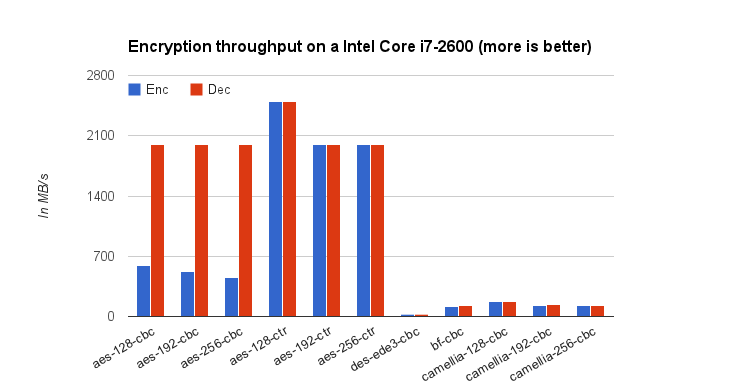
\includegraphics[width=1\textwidth]{benchs-crypto-en.png}\\
Encryption performance in Cloud Gateway
\end{figure}

Encryption is used in two places in Cloud Gateway, first when using an HTTPS endpoint, and when using the encryption filter.

\section{Digest}
\label{sec:performance-digest}

Digest algorithm are used to verify the integrity of files during transfers, if the \textit{Configuration/Instances/Instance/CheckObjectHash}
option is set to true. Almost all providers use the \textit{MD5} algorithm, which has a relatively low CPU-cost.

They are also used to check the integrity of files by comparing the content of objects before they are sent to the provider and after they are retrieved.
This operation is controlled by the \textit{Configuration/Filesystems/FileSystem/InodeDigestAlgorithm} setting, and defaults to use the \textit{SHA-256} digest
algorithm, which is a bit slower than \textit{MD5}. The following picture compares the different algorithms availables on a single core:

\begin{figure}[H]
\centering
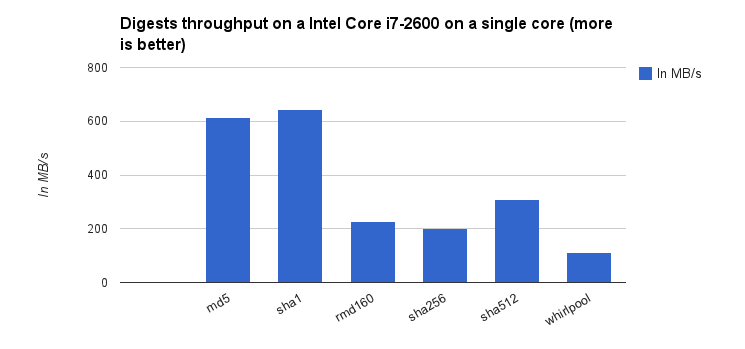
\includegraphics[width=1\textwidth]{benchs-digests-en.png}\\
Digests performance in Cloud Gateway on a single core
\end{figure}

If you want maximum performances and do not care about object integrity, it is possible to disable these two checks.

\section{Compression}
\label{sec:performance-compression}

Compression is a very good way to save bandwidth and storage costs, but it comes with a high impact on CPU processing time
and memory consumption, depending of the compression level chosen. The following benchmark has been realised using a modest Intel Core i7-2600 CPU, on a plain text log file:

\begin{figure}[H]
\centering
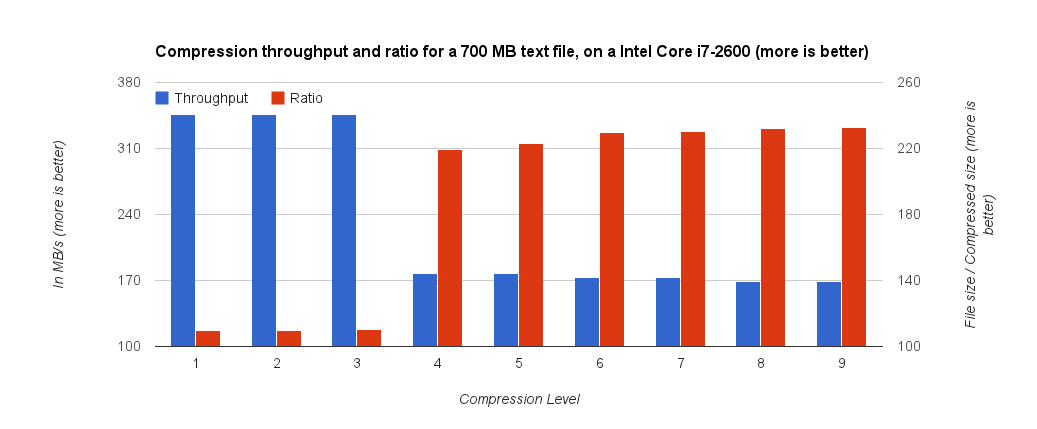
\includegraphics[width=1\textwidth]{benchs-compression-en.png}\\
Compression performance in Cloud Gateway
\end{figure}

\cleardoublepage % Forces the chapter to start on an odd page so it's on the right
\chapter{Command Line Interface}
\label{chap:commnad-line-interface}

\section*{CloudGatewayAddFilesystem}
\label{sec:cloudgatewayaddfilesystem}

This command adds a new filesystem to the Storage Manager configuration file.

\begin{lstlisting}[language=bash]
$ /usr/local/bin/CloudGatewayAddFilesystem
Id, type, cache-root, full-threshold, and file parameters are mandatory.
Usage: CloudGatewayAddFilesystem [OPTIONS] [<instance name>] ...
Required options are:
        -i --id                        Filesystem ID
        -t --type                      Filesystem type, eg Single, Mirroring or Striping
        -c --cache-root                Filesystem cache root directory
        -u --full-threshold            Full Threshold, in percent
        -f --file                      Configuration file
        -m --mount-point               Mount Point
Optional options are:
        -o --io-block-size             Preferred I/O block size, in bytes
        -s --clean-min-file-size       The minimum file size in bytes for an object
                                       to be considered by the cache cleaning process
        -a --clean-max-access-offset   Only files that have been not been accessed for
                                       at least this value (in seconds) might be cleaned
\end{lstlisting}

\subsection*{Parameters}

\begin{itemize}

\item \textbf{Filesystem identifier (-i -{}-id)} the new filesystem's identifier, or name.

\item \textbf{Configuration file (-f -{}-file)} the Cloud Gateway Storage Manager configuration file to update.

\item \textbf{Filesystem type (-t -{}-type)} the new filesystem's type. Three modes are available:
  \begin{itemize}
    \item \textbf{Single}, where the filesystem uses only on instance ;
    \item \textbf{Mirroring}, where data are mirrored on each instance associated with the filesystem ;
    \item \textbf{Striping}, where data are distributed over all instance associated with the filesystem.
  \end{itemize}

\cgconfigreference{Configuration/FileSystems/FileSystem/Type}

\item \textbf{Cache root (-c -{}-cache-root)} the root cache directory of the new filesystem.

\cgconfigreference{Configuration/FileSystems/FileSystem/CacheRoot}

\item \textbf{Full threshold (-u -{}-full-threshold)} the full threshold of the new filesystem, over which the cleaner begins to expunge cache entries.

\cgconfigreference{Configuration/FileSystems/FileSystem/FullThreshold}

\item \textbf{I/O block size (-o -{}-io-block-size)} the new filesystem's preferred I/O block size, in bytes.

\cgconfigreference{Configuration/FileSystems/FileSystem/IOBlockSize}

\item \textbf{Cleaner minimum file size (-s -{}-clean-min-file-size)} the new filesystem's cleaner minimum file size. Files smaller than this size won't get expunged from the cache.

\cgconfigreference{Configuration/FileSystems/FileSystem/CleanMinFileSize}

\item \textbf{Cleaner maximum access offset (-a -{}-clean-max-access-offset)} the new filesystem's cleaner maximum offset. Only files that have not been accessed for at least as many seconds are considered for cleaning.

\cgconfigreference{Configuration/FileSystems/FileSystem/CleanMaxAccessOffset}

\item \textbf{Configuration file (-m -{}-mount-point)} the mount point where the filesystem will be mounted.

\end{itemize}

\clearpage

\section*{CloudGatewayAddFilterToInstance}
\label{sec:cloudgatewayaddfiltertoinstance}

This command adds a filter to an existing instance.

\begin{lstlisting}[language=bash]
$ /usr/local/bin/CloudGatewayAddFilterToInstance
Name, type and file parameters are mandatory.
Usage: CloudGatewayAddFilterToInstance [OPTIONS]
Required options are:
        -i --instance-name                       Instance name
        -t --type                                Filter type (Compression, Encryption)
        -f --file                                Configuration file
Optional options are:
        -l --level                               Compression Level (required for
                                                 Compression filter)
        -c --cipher                              Cipher (required for Encryption filter)
        -d --digest                              Digest used to derive an encryption key
                                                 (required for Encryption filter)
        -k --key-iteration-count                 Count of iterations used to derive an encryption
                                                 key (required for Encryption filter)
        -p --password                            Password used to derive an encryption key
                                                 (required for Encryption filter)
Please look at the product documentation for more information.
\end{lstlisting}

\subsection*{Parameters}

\begin{itemize}
\item \textbf{Instance identifier (-i -{}-id)} the existing instance's name.

\item \textbf{Configuration file (-f -{}-file)} the Cloud Gateway Storage Manager configuration file to update.

\item \textbf{Filter type (-t -{}-type)} the new filter's type. Two filter types are available:
  \begin{itemize}
    \item \textbf{Compression}, compressing file content on-the-fly before sending it to the Cloud ;
    \item \textbf{Encryption}, encrypting file content on-the-fly before sending it to the Cloud.
  \end{itemize}

\cgconfigreference{Configuration/Instances/Instance/Filters/Filter/Type}

\item \textbf{Level (-l -{}-level)} the compression level used by the compression filter. Valid levels range from 1 to 9, 1 being the fastest and 9 the most efficient, albeit slowest and memory consuming.

\cgconfigreference{Configuration/Instances/Instance/Filters/Filter/Specifics/Level}

\item \textbf{Cipher (-c -{}-cipher)} the cipher used by the encryption filter.

\cgconfigreference{Configuration/Instances/Instance/Filters/Filter/Specifics/Cipher}

\item \textbf{Digest (-d -{}-digest)} the digest used to derive an encryption key from the password, with the encryption filter.

\cgconfigreference{Configuration/Instances/Instance/Filters/Filter/Specifics/Digest}

\item \textbf{Key iteration count (-k -{}-key-iteration-count)} the number of iterations used to derive an encryption key from the password, with the encryption filter.

\cgconfigreference{Configuration/Instances/Instance/Filters/Filter/Specifics/KeyIterationCount}

\item \textbf{Password (-p -{}-password)} the password used to derive an encryption key, with the encryption filter.

\cgconfigreference{Configuration/Instances/Instance/Filters/Filter/Specifics/Password}

\end{itemize}

\clearpage

\section*{CloudGatewayAddInstance}
\label{sec:cloudgatewayaddinstance}

This command adds a new instance to the Storage Manager configuration file.

\begin{lstlisting}[language=bash]
$ /usr/local/bin/CloudGatewayAddInstance
Name, provider and file parameters are mandatory.
Usage: CloudGatewayAddInstance [OPTIONS]
Required options are:
        -n --name                                Instance name
        -P --provider                            Provider type (Amazon, Openstack)
        -f --file                                Configuration file
Optional options are:
        -a --access-key-id                       Access Key ID (required for type Amazon)
        -s --secret-access-key                   Secret Access Key (required for type Amazon)
        -e --endpoint                            Endpoint (required for type Amazon)
        -g --endpoint-port                       Endpoint port (required for type Amazon)
        -b --bucket                              Bucket (required for type Amazon)
        -S --secure-transaction                  Whether to use HTTPs (required for Amazon)
        -i --identity-version                    Identity Version for Openstack (required for Openstack)
        -u --user-name                           Username (required for Openstack)
        -p --password                            Password (required for Openstack v2)
        -t --tenant-id                           Tenant ID
        -T --tenant-name                         Tenant Name
        -I --api-access-key                      API Access Key (required for Openstack v1)
        -A --authentication-endpoint             Authentication Endpoint (required for Openstack)
        -c --container                           Container (required for Openstack)
        -r --preferred-region                    Preferred region to use with Openstack, if any
        -m --authentication-max-life-time        Authentication max lifetime for an Openstack token
        -R --authentication-token-recent-delay   An Openstack authentication error with a token older than
                                                 this delay will trigger a re-authentication
        -k --allow-insecure                      Allow insecure (invalid certificate) communication
Please look at the product documentation for more information.
\end{lstlisting}

\subsection*{Parameters}

\begin{itemize}
\item \textbf{Instance name (-n -{}-name)} the new instance's name, or identifier.

\item \textbf{Configuration file (-f -{}-file)} the Cloud Gateway Storage Manager configuration file to update.

\item \textbf{Provider type -P -{}-provider} the new instance's provider type, two types are available:
  \begin{itemize}
    \item \textbf{Amazon}, all providers compatible with the S3 API ;
    \item \textbf{Openstack}, all providers compatible with the Openstack Swift API.
  \end{itemize}

\cgconfigreference{Configuration/Instances/Instance/Provider}

\item \textbf{Access key identifier (-a -{}-access-key-id)} the access key identifier, required when using a S3 provider.

\cgconfigreference{Configuration/Instances/Instance/Specifics/AccessKeyId}

\item \textbf{Secret access key (-s -{}-secret-access-key)} the secret access key, required when using a S3 provider.

\cgconfigreference{Configuration/Instances/Instance/Specifics/SecretAccessKey}

\item \textbf{Endpoint (-e -{}-endpoint)} the cloud provider endpoint, required when using a S3 provider.

\cgconfigreference{Configuration/Instances/Instance/Specifics/Endpoint}

\item \textbf{Endpoint port (-g -{}-endpoint-port)} the cloud provider endpoint port, required when using a S3 provider.

\cgconfigreference{Configuration/Instances/Instance/Specifics/EndpointPort}

\item \textbf{Bucket (-b -{}-bucket)} an existing bucket to use, required when using a S3 provider.

\cgconfigreference{Configuration/Instances/Instance/Specifics/Bucket}

\item \textbf{Secure transaction (-S -{}-secure-transaction)} whether to use SSL/TLS to secure transfers, required when using a S3 provider.

\cgconfigreference{Configuration/Instances/Instance/Specifics/SecureTransaction}

\item \textbf{Identity version (-i -{}-identity-version)} the Openstack Swift identity version to use, required when using an Openstack provider.

\cgconfigreference{Configuration/Instances/Instance/Specifics/IdentityVersion}

\item \textbf{Username (-u -{}-user-name)} the username used to authenticate to the storage provider, required when using an Openstack provider.

\cgconfigreference{Configuration/Instances/Instance/Specifics/Username}

\item \textbf{Password (-p -{}-password)} the password used to authenticate to the storage provider, required when using an Openstack provider and identity v2.

\cgconfigreference{Configuration/Instances/Instance/Specifics/Password}

\item \textbf{Tenant ID (-t -{}-tenant-id)} the tenant ID used to authenticate to the storage provider, required when using an Openstack provider and identity v2 with a tenant ID.

\cgconfigreference{Configuration/Instances/Instance/Specifics/TenantId}

\item \textbf{Tenant name (-T -{}-tenant-name)} the tenant name used to authenticate to the storage provider, required when using an Openstack provider and identity v2 with a tenant name.

\cgconfigreference{Configuration/Instances/Instance/Specifics/TenantName}

\item \textbf{API access key (-I -{}-api-access-key)} the API access key used to authenticate to the storage provider, required when using an Openstack provider and identity v1.

\cgconfigreference{Configuration/Instances/Instance/Specifics/APIAccessKey}

\item \textbf{Authentication endpoint (-A -{}-authentication-endpoint)} the cloud storage provider authentication endpoint, required when using an Openstack provider.

\cgconfigreference{Configuration/Instances/Instance/Specifics/AuthenticationEndpoint}

\item \textbf{Container (-c -{}-container)} an existing container to use, required when using an Openstack provider.

\cgconfigreference{Configuration/Instances/Instance/Specifics/Container}

\item \textbf{Preferred region (-r -{}-preferred-region)} the preferred region to use, if any, when using an Openstack provider.

\cgconfigreference{Configuration/Instances/Instance/Specifics/PreferredRegion}

\item \textbf{Authentication maximum lifetime (-m -{}-authentication-max-life-time)} the maximum lifetime of an Openstack token.

\cgconfigreference{Configuration/Instances/Instance/Specifics/AuthenticationMaxLifetime}

\item \textbf{Authentication recent token delay (-R -{}-authentication-recent-token-delay)} authentication error when using an Openstack token older than this delay will trigger a re-authentication attempt.

\cgconfigreference{Configuration/Instances/Instance/Specifics/AuthenticationTokenRecentDelay}

\item \textbf{Allow insecure connection (-k -{}-allow-insecure)} allows the cloud provider to present an invalid certificate. This means that the transfer will not be secured.

\cgconfigreference{Configuration/Instances/Instance/Specifics/AllowInsecureHTTPS}

\end{itemize}

\clearpage

\section*{CloudGatewayListFilesystems}
\label{sec:cloudgatewaylistfilesystems}

This command lists all filesystems (also known as volumes) present in the given configuration file.

\begin{lstlisting}[language=bash]
$ /usr/local/bin/CloudGatewayListFilesystems
File parameter is mandatory.
Usage: CloudGatewayListFilesystems [OPTIONS]
Required options are:
        -f --file                                Configuration file
Please look at the product documentation for more information.
\end{lstlisting}

\subsection*{Parameters}

\begin{itemize}
\item \textbf{Configuration file (-f -{}-file)} the Cloud Gateway Storage Manager configuration file to read information from.

\end{itemize}

\clearpage

\section*{CloudGatewayListInstances}
\label{sec:cloudgatewaylistinstances}

This command lists all instances existing in the given configuration file.

\begin{lstlisting}[language=bash]
$ /usr/local/bin/CloudGatewayListInstances
File parameter is mandatory.
Usage: CloudGatewayListInstances [OPTIONS]
Required options are:
        -f --file                                Configuration file
Please look at the product documentation for more information.
\end{lstlisting}

\subsection*{Parameters}

\begin{itemize}
\item \textbf{Configuration file (-f -{}-file)} the Cloud Gateway Storage Manager configuration file to read information from.

\end{itemize}

\clearpage

\section*{CloudGatewayMount}
\label{sec:cloudgatewaymount}

This command mounts the filesystem (also known as volume) specified in the given configuration file.

\begin{lstlisting}[language=bash]
$ /usr/local/bin/CloudGatewayMount
Usage: $0 [<Mount point>] <Configuration File>
\end{lstlisting}

\subsection*{Parameters}

\begin{itemize}
\item \textbf{Mount point} the directory where the filesystem should be mounted. This is only required if the \textit{MountPoint} value does not exist in the configuration file.

\cgconfigreference{Configuration/FileSystems/FileSystem/MountPoint}

\item \textbf{Configuration file} the mount point configuration file.

\end{itemize}

\clearpage

\section*{CloudGatewayMountConfigTest}
\label{sec:cloudgatewaymountconfigtest}

This command parses the given filesystem configuration file, in order to verify that it is valid.

\begin{lstlisting}[language=bash]
$ /usr/local/bin/CloudGatewayMountConfigTest
CloudGatewayMountConfigTest <Cloud Gateway mount configuration file>
\end{lstlisting}

\subsection*{Parameters}

\begin{itemize}

\item \textbf{Configuration file} the mount point configuration file.

\end{itemize}

\clearpage

%\section*{CloudGatewayNFSAddClient}
%\section*{CloudGatewayNFSAddExport}
%\section*{CloudGatewayNFSControl}
%\section*{CloudGatewayNFSRemoveClient}
%\section*{CloudGatewayNFSRemoveExport}
%\section*{CloudGatewayNFSShowXml}

\section*{CloudGatewayRemoveFilesystem}
\label{sec:cloudgatewayremovefilesystem}

This command removes an existing filesystem definition from the Cloud Gateway configuration file.

\begin{lstlisting}[language=bash]
$ /usr/local/bin/CloudGatewayRemoveFilesystem
Name, type and file parameters are mandatory.
Usage: CloudGatewayRemoveFilesystem [OPTIONS]
Required options are:
        -i --id                                  Filesystem ID
        -f --file                                Configuration file
Please look at the product documentation for more information.
\end{lstlisting}

\subsection*{Parameters}

\begin{itemize}
\item \textbf{Filesystem identifier (-i -{}-id)} the name of the filesystem (or volume) to remove.

\item \textbf{Configuration file (-f -{}-file)} the Cloud Gateway Storage Manager configuration file to update.

\end{itemize}

\clearpage

\section*{CloudGatewayRemoveFilterFromInstance}
\label{sec:cloudgatewayremovefilterfrominstance}

This command removes an existing filter associated to an instance from the Cloud Gateway configuration file.

\begin{lstlisting}[language=bash]
$ /usr/local/bin/CloudGatewayRemoveFilterFromInstance
Name, type and file parameters are mandatory.
Usage: CloudGatewayRemoveFilterFromInstance [OPTIONS]
Required options are:
        -i --instance-name                       Instance name
        -t --type                                Filter type (Compression, Encryption)
        -f --file                                Configuration file
Please look at the product documentation for more information.
\end{lstlisting}

\subsection*{Parameters}

\begin{itemize}
\item \textbf{Instance identifier (-i -{}-instance-name)} the name of the instance whose filter has to be removed.

\item \textbf{Filter type (-f -{}-type)} the type of the filter to be removed.

\cgconfigreference{Configuration/Instances/Instance/Filters/Filter/Type}

\item \textbf{Configuration file (-f -{}-file)} the Cloud Gateway Storage Manager configuration file to update.

\end{itemize}

\clearpage

\section*{CloudGatewayRemoveInstance}
\label{sec:cloudgatewayremoveinstance}

This command removes an existing instance from the Cloud Gateway configuration file.

\begin{lstlisting}[language=bash]
$ /usr/local/bin/CloudGatewayRemoveInstance
Name and file parameters are mandatory.
Usage: CloudGatewayRemoveInstance [OPTIONS]
Required options are:
        -i --instance-name                       Instance name
        -f --file                                Configuration file
Please look at the product documentation for more information.
\end{lstlisting}

\subsection*{Parameters}

\begin{itemize}
\item \textbf{Instance identifier (-i -{}-instance-name)} the name of the instance to remove.

\item \textbf{Configuration file (-f -{}-file)} the Cloud Gateway Storage Manager configuration file to update.

\end{itemize}

\clearpage

\section*{CloudGatewayShowFilesystem}
\label{sec:cloudgatewayshowfilesystem}

This command displays a filesystem's configuration.

\begin{lstlisting}[language=bash]
$ /usr/local/bin/CloudGatewayShowFilesystem
Id and file parameters are mandatory.
Usage: CloudGatewayShowFilesystem [OPTIONS]
Required options are:
        -i --id                                  Filesystem ID
        -f --file                                Configuration file
Please look at the product documentation for more information.
\end{lstlisting}

\subsection*{Parameters}

\begin{itemize}
\item \textbf{Filesystem identifier (-i -{}-id)} the filesystem identifier.

\item \textbf{Configuration file (-f -{}-file)} the Cloud Gateway Storage Manager configuration file.

\end{itemize}

\clearpage

\section*{CloudGatewayShowInstance}
\label{sec:cloudgatewayshowinstance}

This command displays an instance's configuration.

\begin{lstlisting}[language=bash]
$ /usr/local/bin/CloudGatewayShowInstance
Name and file parameters are mandatory.
Usage: CloudGatewayShowInstance [OPTIONS]
Required options are:
        -i --instance-name                       Instance name
        -f --file                                Configuration file
Please look at the product documentation for more information.
\end{lstlisting}

\subsection*{Parameters}

\begin{itemize}
\item \textbf{Instance identifier (-i -{}-instance-name)} the instance name.

\item \textbf{Configuration file (-f -{}-file)} the Cloud Gateway Storage Manager configuration file.

\end{itemize}

\clearpage

\section*{CloudGatewayShowMount}
\label{sec:cloudgatewayshowmount}

This command displays a mount point configuration.

\begin{lstlisting}[language=bash]
$ /usr/local/bin/CloudGatewayShowMount
File parameter is mandatory.
Usage: CloudGatewayShowMount [OPTIONS]
Required options are:
        -f --file                                Configuration file
Please look at the product documentation for more information.
\end{lstlisting}

\subsection*{Parameters}

\begin{itemize}
\item \textbf{Configuration file (-f -{}-file)} the mount point configuration file.

\end{itemize}

\clearpage

\section*{CloudGatewayStatus}
\label{sec:cloudgatewaystatus}

This command displays the number of files (and optionally the status of each one) that are not synchronised
with the cloud storage provider, either because they have been modified (dirty state) or deleted, and the
modification has not been repercuted to the storage provider yet.

\begin{lstlisting}[language=bash]
$ /usr/local/bin/CloudGatewayStatus
\end{lstlisting}

\subsection*{Parameters}

\begin{itemize}
\item \textbf{Verbose (-v)} displays the status of each deleted or dirty file.

\end{itemize}

\clearpage

\section*{CloudGatewayStorageManager}
\label{sec:cloudgatewaystoragemanager}

This command controls the Cloud Gateway Storage Manager.

\begin{lstlisting}[language=bash]
$ /usr/local/bin/CloudGatewayStorageManager
Usage: /usr/local/bin/CloudGatewayStorageManager \
  [start|stop|graceful-stop|force-stop|restart|reload|status
\end{lstlisting}

\subsection*{Options}

\begin{itemize}
\item \textbf{start} Start the Storage Manager.

\item \textbf{stop} Stop the Storage Manager using a graceful stop. See \nameref{sec:graceful-stop-and-force-stop} on page~\pageref{sec:graceful-stop-and-force-stop}.

\item \textbf{graceful-stop} Gracefully stop the Storage Manager. See \nameref{sec:graceful-stop-and-force-stop} on page~\pageref{sec:graceful-stop-and-force-stop}.

\item \textbf{force-stop} Alias for graceful-stop.

\item \textbf{restart} Stop the Storage Manager using a force stop, then start it.

\item \textbf{reload} Gracefully reload Storage Manager. See \nameref{sec:graceful-reload} on page~\pageref{sec:graceful-reload}.

\item \textbf{status} Print whether the Storage Manager is running or not.

\end{itemize}

\clearpage

\section*{CloudGatewayStorageManagerConfigTest}
\label{sec:cloudgatewaystoragemanagerconfigtest}

This command parses the given Storage Manager configuration file, in order to verify that it is valid.

\begin{lstlisting}[language=bash]
$ /usr/local/bin/CloudGatewayStorageManagerConfigTest
CloudGatewayStorageManagerConfigTest <Cloud Gateway Storage Manager configuration file>
\end{lstlisting}

\subsection*{Parameters}

\begin{itemize}

\item \textbf{Configuration file} the Storage Manager configuration file.

\end{itemize}

\clearpage

\section*{CloudGatewayStorageManagerUnMount}
\label{sec:cloudgatewaystoragemanagerunmount}

This command unmounts the filesystem (also known as volume) specified in the given configuration file.

\begin{lstlisting}[language=bash]
$ /usr/local/bin/CloudGatewayUnmount
Usage: /usr/local/bin/CloudGatewayUnmount [<Mount point>|<Configuration File>]
\end{lstlisting}

\subsection*{Parameters}

\begin{itemize}
\item \textbf{Mount point} the directory where the filesystem is mounted.

\cgconfigreference{Configuration/FileSystems/FileSystem/MountPoint}

\item \textbf{Configuration file} the mount point configuration file.

\end{itemize}

\clearpage

\chapter{Configuration Options}
\label{chap:configuration-options}

\section{Storage Manager Configuration Options}
\label{sec:storage-manager-configuration-options}

This section contains the documentation of all the parameters supported by Cloud Gateway Storage Manager in its configuration file, located at \textit{/usr/local/etc/CloudGatewayConfiguration.xml}.

\input{./CloudGatewayStorageManagerConfiguration.tex}

\end{document}
